\documentclass[12pt]{paper}
\textwidth=17cm
\textheight=23.5cm
\usepackage[utf8]{inputenc}
\usepackage[spanish]{babel}
\usepackage{amsmath,amssymb,exscale,graphicx}
%\input epsf
\parskip 0.3cm
\usepackage{bm}


\title{\begin{center}Bayesian Statistics and Machine Learning Workshop 2023\end{center}}
\subtitle{\begin{center}\Large Fundamentals of Bayesian statistics\\ Martín Onetto \end{center}}

\begin{document}
\maketitle


\topmargin -2.0cm
\oddsidemargin -0.2cm
\evensidemargin -0.2cm

\vspace{-80pt}
%This practice is intended for your own exercise and {\bf does not} need to be turned in. 

\section{Questions}

\begin{enumerate}
\item Discutir qué significa la probabilidad de una afirmación o evento.
\item Cómo se representa cuantitativamente que una afirmación es asbolutamente cierta?
\item Crear un ejemplo donde hay dos proposiciones lógicas y se cumpla un silogismo fuerte.
\item Relacionar la lógica de bool con las operacione ssuma y multiplicación de proposiciones lógica
\item Discutir qué representa conceptualmente la marginalización.
\item Deducir el Teorema de Bayes de la regla del producto.
\end{enumerate}
\newpage
\section{Problems}

\begin{enumerate}
\item Resolver el problema de Monty Hall y programarlo en python.
\item Ver cómo cambia la probabilidad de ganar el premio a medida que se agregan puertas (siempre Monty abre $N-2$ puertas)

\item Las hormigas recorren el laberinto mostrado en la figura en direccion descendente, siguiendo las flechas. Ingresan por arriba (entradas $a_{1}$ y $a_{2}$, ambas equiprobables) y salen por abajo (salidas $b_{1}$ y $b_{2}$). En cada bifurcacion (los lugares donde hay que decidir si avanzar hacia la derecha o hacia la izquierda, marcados con flechas negras del dibujo), la probabilidad de virar a la izquierda es de $1/3$, y la de la derecha, $2/3$. Calcule la probabilidad de que una hormiga haya entrado por $a_{1}$,si sabemos que sale por $b_{1}$.
\begin{figure}[ht]
    \centering
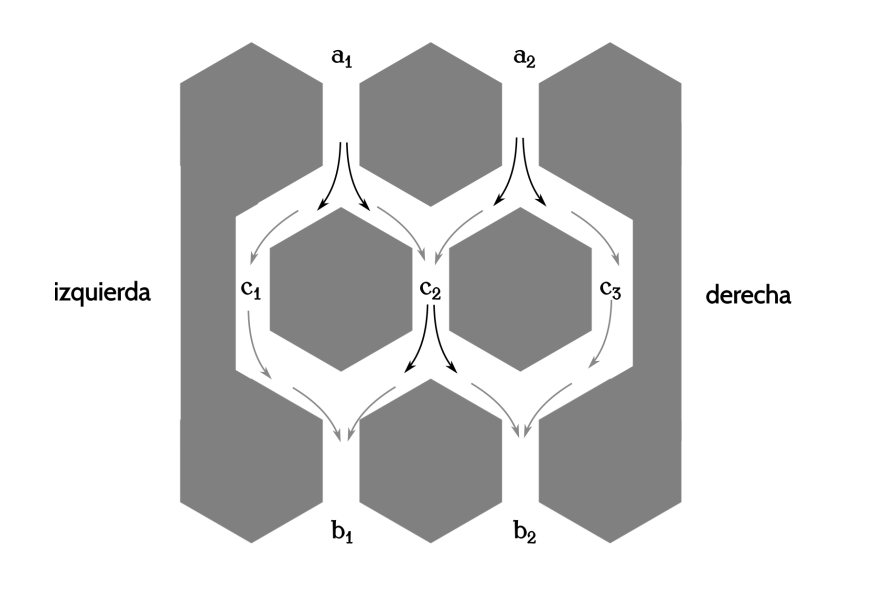
\includegraphics[width=0.6\textwidth]{bin/figs/laberint.png}
    \label{fig:lab}
\end{figure}
\item Simular el problema anterior y graficar los histogramas que representan las probabilidades calculadas.

\end{enumerate}

\pagestyle{empty}

\end{document}
